\documentclass[main.tex]{subfiles}
\begin{document}
\onlyinsubfile{\mainmatter{}}

\chapter{Glyco: A Nanopass Compiler for CHERI-RISC-V} \label{ch:glyco}
Glyco\footnote{From the Greek term $\gamma\lambda\upsilon\kappa{}\text{ò}$ meaning \enquote{sweet}, alluding to the taste of a wild cherry.} is a compiler targeting the CHERI-RISC-V architecture, producing software running on CheriBSD systems and on a Sail-based emulator of the CHERI-RISC-V ISA.

Glyco follows a \g{nanopass} compiler design, an iterative approach to designing and implementing a compiler that results in a series of transformations of a program from a high-level language to a low-level language (such as assembly) via several intermediate languages. We briefly discuss this approach in \cref{sct:nanopass}. The languages in Glyco are summarised in \cref{fig:pipeline01}.

\begin{figure}
	\centering
	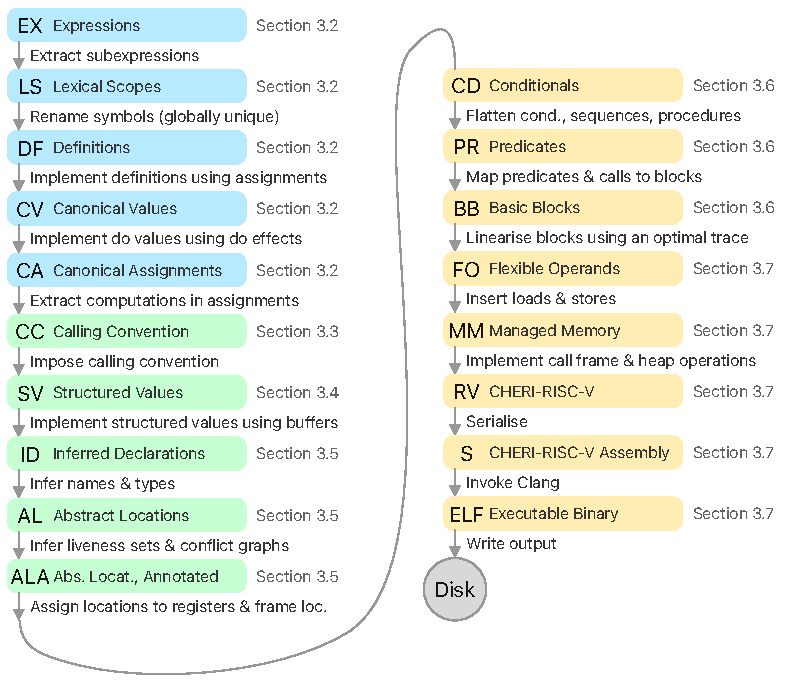
\includegraphics{Images/Pipeline v0.1.pdf}
	\caption{The Glyco 0.1 pipeline, consisting (from top to bottom) of high-level (blue), mid-level (green), and low-level (orange) languages. The informal partition of the pipeline in three segments is mostly based on how much access to physical locations (such as registers) a language provides.}
	\label{fig:pipeline01}
\end{figure}

In \cref{sct:ex} we discuss the high-level \textbf{Expressions} language (EX), a functional programming language with support for common features such as functions, conditionals, definitions, vectors, and records. These features are implemented in several transformations from EX to the CC language.

The \textbf{Calling Convention} language (CC) is a procedural programming language with support for procedures, variables, conditionals, vectors, and records. It is the lowest language in Glyco that supports the notion of a procedure with parameters and results. CC programs are transformed to SV programs by imposing a set of rules governing procedure calls, i.e., a \g{cc}. We discuss \gs{cc} and the CC language in \cref{sct:cc}.

\textbf{Structured Values} (SV) is a structured imperative programming language with support for variables, conditionals, vectors, and records, and is discussed in \cref{sct:sv}. It is so named because it is the lowest abstraction that supports structured values, i.e., vectors and records, as opposed to untyped byte buffers. SV programs are transformed to ID programs by substituting indices and fields with byte offsets.

\textbf{Inferred Declarations} (ID), \textbf{Abstract Locations} (AL), and \textbf{Abstract Locations Annotated} (ALA) are three structured imperative languages with support for variables and conditionals; all three are discussed in \cref{sct:id}. ID programs do not need to declare local variables whereas AL programs do need to declare them. The transformation between the two languages performs a basic inference algorithm to discover the names and types of variables. AL programs are then \lowered{} to ALA programs which contain additional liveness and conflict information. This information is then used to perform register allocation and assign a register or memory location to each variable, resulting in a CD program.

In \cref{sct:cd} we go over \textbf{Conditionals} (CD), a structured imperative language with support for conditionals. CD programs are flattened over several passes to \textbf{Flexible Operands} (FO) programs, which consist of labelled and unlabelled effects in a similar way to labelled and unlabelled instructions in an assembly program. We then tackle the last few languages and transformations in \cref{sct:fo} that finally produce an ELF executable.

This chapter discusses the feature set and languages of Glyco 0.1,\footnote{The source code is available at \url{https://tsarouhas.eu/glyco/0.1/}.} which allows us to focus in each chapter on one set of functionality. It also permits us to evaluate how the nanopass approach performs with extensions in future versions which we discuss in later chapters.

Example programs in this chapter follow the syntax of the final version of the compiler, Glyco 1.0,\footnote{The source code is available at \url{https://tsarouhas.eu/glyco/1.0/}.} and are compiled using the default configuration. The syntax of a program in one compiler version does not significantly change in another version but for consistency we chose to express all programs in the latest compiler's syntax, skipping languages introduced after Glyco 0.1. A full language reference of this syntax can be found in \cref{ch:grammar}. 

\section{Background: Nanopass Compilers} \label{sct:nanopass}
Glyco is built following a \emph{nanopass} compiler design, described in the context of compiler education \citep{educomp} and commercial compiler development \citep{commcomp}. A nanopass compiler consists of numerous small passes, so-called \textbf{\glspl{nanopass}}, which translate programs written in one \textbf{\g{il}} to programs written in another. The input of a \g{nanopass} is a program in a higher-level language than the one of its output; we therefore call this translation process a \textbf{\g{lowering}}. A \g{nanopass} should be concise and perform a relatively self-contained transformation. There should be no data structures shared across \gs{nanopass} except for the program itself.

The nanopass design allows the compiler engineer to design and implement their compiler \emph{by iterated abstraction}. A simplified description follows. The engineer first chooses a target language (usually a machine language such as x86-64 or indeed CHERI-RISC-V) and determines an abstraction over it. The engineer then defines an \g{il} that implements that abstraction as well as a \gls{nanopass} which transforms programs written in the new \g{il} to the target language. The compiler engineer then repeats this process, this time abstracting over the \g{il} with a new \g{il} and \gls{nanopass}. This process goes on until a level of abstraction has been reached that can either be directly used as a source language (by human users), or be easily produced by parser actions.

An important benefit of the nanopass approach is each new iteration begins and ends with a working compiler. After each iteration, users can start writing and compiling programs in the new \g{il} and unit tests can be written that ensure that the new \gls{nanopass} produces the expected transformations. For experimental architectures such as CHERI-RISC-V, this also means that designers can experiment more quickly with new ideas, something that may be harder to do on a full-fledged production compiler such as Clang.

Glyco 0.1 defines 17 \gs{il},\footnote{We don't consider ELF to be an \g{il} in this thesis.} a majority of which are adapted from the student compiler by \citet{compcourse} for x86 targets. Each language is usually named after the new abstraction or feature it brings compared to the \g{lowerlang}. We discuss the \gs{il} in reverse chronological order (from high-level to low-level languages) as opposed to the order in which the \gs{il} were defined (from low-level to high-level languages). This allows us to explain the compiler pipeline using example programs, showing how they are manipulated by the compiler's \gs{nanopass}.

\newpage

\section{An Expression Language} \label{sct:ex}
\plfig[11]{v0.1 EX}

This section introduces the EX, LS, DF, CV, and CA languages. The \gs{nanopass} between these \gs{il} consecutively transform programs from a functional to an imperative, procedural language.

The highest \g{il} in the first version of Glyco is called \textbf{EX} (Expressions), a language with basic support for arithmetic operations, functions, conditionals (\texttt{if}-\texttt{then}-\texttt{else}), definitions (\texttt{let}-bindings), vectors (fixed-size arrays), and records (collections of key-value pairs).

The following EX program computes the 30th number in the Fibonacci sequence starting with 0 and 1:\footnote{EX and all other \gs{il} conform to the Sisp format, where a list is written as the list's elements separated by whitespace and where attributes are separated by commas. Sisp is briefly documented in \cref{ch:sisp}.}
\ilfile{Programs/fib.ex}

This program defines a function \iil/fib/ with three signed 32-bit integer parameters \iil/prev/, \iil/curr/, and \iil/iter/ which returns a signed 32-bit integer. The function recursively adds the \enquote{previous} and \enquote{current} sums until the number of iterations drops to 0, then returns the \enquote{current} sum. The program itself is defined as the result of \iil/fib/ where \iil/prev/ is 0, \iil/curr/ is 1, and \iil/iter/ is 30.

EX is an \emph{intermediate} language and not necessarily a \emph{user-friendly} language; it contains little syntactical sugar. For example, the predicate $ \textit{iter} \le 1 $ is written as \iil/relation(iter, le, 1)/. A significant benefit is that the structure is easy to manipulate as the code goes through the compiler's \gs{nanopass}. One can however define a more user-friendly language and write a parser that emits EX.

\paragraph{From EX to LS} LS (Lexical Scopes) does not support subexpressions so the \g{nanopass} to LS binds all subexpressions to names (temporaries) and uses those names in place of the subexpressions. For instance, the EX value
\begin{il}
	evaluate(function(fib), ... binary(prev, add, curr) ...)
\end{il}
is transformed into the equivalent LS value
\begin{il*}{samepage=true}
	let(
		(arg0, ...) (arg1, let(
			(ex.lhs, source(prev)) (ex.rhs, source(curr)),
			in: binary(ex.lhs, add, ex.rhs)
		)) (arg2, ...),
		in: evaluate(function(fib), arg0 arg1 arg2)
	)
\end{il*}

Some transformations are not strictly necessary, e.g., binding \iil/prev/ to \iil/ex.lhs/ instead of using \iil/prev/ directly. They do not however incur any additional overhead in the final executable: a \g{nanopass} further down the compiler pipeline cleans up these redundant temporaries.

\paragraph{From LS to DF} DF (Definitions) does not support shadowing; all \texttt{let} bindings are in a single namespace. The \g{nanopass} from LS to DF implements shadowing by renaming symbols such that each definition uses a globally unique symbol.

\paragraph{From DF to CV} CV (Canonical Values) does not support \texttt{let} bindings, i.e., definitions. The \g{nanopass} implements each definition in CV using a \texttt{do} value, i.e., a computed value, a value on which a computation can be attached, with a \texttt{set} effect in it. For example, the DF value
\begin{il}
	let((answer, source(42)), in: source(answer))
\end{il}
is \lowered{} to the CV value
\begin{il}
	do(set(answer, to: source(42)), then: source(answer))
\end{il}

\paragraph{From CV to CA} CA (Canonical Assignments) does not support \texttt{do} \emph{values}, but does support \texttt{do} \emph{effects}, which are sequences of effects. The \g{nanopass} implements \texttt{do} values by extracting their effects into \texttt{do} effects and ending with an additional \texttt{set} effect that moves the result to the intended destination. That is, a CV \texttt{set} effect
\begin{il}
	set(result, to:
		do(
			/* effects */,
			then: /* result */
		)
	)
\end{il}
is transformed to a CA \texttt{do} effect
\begin{il}
	do(
		/* effects */
		set(result, to: /* result */)
	)
\end{il}

\paragraph{From CA to CC} CA programs perform assignments using \texttt{set} effects, whereas CC (Calling Convention) only supports \texttt{set} effects with a constant or location source, and provides other effects that perform more complicated tasks such as allocating records. The final purely structural transformation lowers \texttt{set} effects in CA using equivalent effects in CC. For example, the CA program
\ilfile{Programs/values.ca}
is \lowered{} to the CC program
\ilfile{Programs/values.cc}

\section{A Conventional Calling Convention} \label{sct:cc}
\plfig[4]{v0.1 CC}

This section introduces \gs{cc}, the CC language, and its associated \g{nanopass}.

A \textbf{\g{cc}} is a set of rules imposed by the operating system, instruction set architecture, and/or programming language that specify how procedures are called. A low-level \g{cc} often specifies
\begin{itemize}[noitemsep]
	\item where parameters and result values are placed (in dedicated registers, in a particular order on the call stack, or a combination of both);
	\item how large values are passed to the callee or caller (over multiple registers, on the call stack, or in heap memory), if supported;
	\item the state of the call stack and some registers (like the register keeping the frame pointer) when a procedure starts executing and when it returns to the caller;
	\item which registers a procedure can use freely but for which it cannot assume that their contents will be preserved across a procedure call (\textbf{\gs{cersaved}}); and
	\item which registers a procedure can only use after saving their previous contents and if they're restored after use (\textbf{\gs{ceesaved}}).
\end{itemize}

The \g{cc} used in the base version of Glyco is called \textbf{\g{gccc}} and mimics a traditional \g{cc} that would be used for programs written in C, with some parts specified by \cite[chapter~25]{riscv}.

\paragraph{Call stack} The call stack is a region of memory on which information about procedure calls is stored, such as local state and return addresses. The stack grows downward, i.e., from high to low addresses. The \texttt{csp} register contains the \textbf{\g{stackcap}}, a capability that points to the location of the last pushed datum, i.e., the top of the stack, and gives read-write authority over the stack memory. The \g{stackcap}'s address decreases whenever data are pushed to the call stack and increases whenever data are popped from the stack.

\paragraph{Call frames} A call frame (also known as a \emph{stack frame}) is a region of memory on the call stack that belongs to a procedure call and on which the procedure can store its local state. The \texttt{cfp} register contains the \textbf{\g{framecap}}, a capability derived from the \g{stackcap} that points to the base of the call frame. The procedure places local state and expects parameters in locations that are fixed distances removed from this base.

Before accessing its call frame, a procedure pushes a call frame of the desired size to the call stack in three steps. The procedure first pushes the (caller's) \g{framecap} to the call stack, then updates the \g{framecap} to point to this capability, and finally allocates room for its local state by moving the \g{stackcap} so that it points to the new call frame's last datum.

A procedure pops its call frame when it is done using it, e.g., when returning to its caller. It does so by popping all data stored in the call frame and restoring the previous \g{framecap}.

\paragraph{Parameters} Arguments to parameters are passed to the callee via dedicated argument registers first. When the set of argument registers is exhausted, any remaining arguments are pushed (in order) to the stack where they become part of the caller's call frame for the duration of the call.\footnote{This is the only part of another procedure's call frame that a callee is allowed to access directly.} Since these \emph{frame-resident} arguments reside at higher addresses than the callee's \g{framecap}, the callee can access these arguments using positive offsets of the \g{framecap}.

The set of argument parameters in Glyco is customisable via a command-line option. The default set is \texttt{a0}, \texttt{a1}, \texttt{a2}, \texttt{a3}, \texttt{a4}, \texttt{a5}, \texttt{a6}, and \texttt{a7}.

All of Glyco's supported data types in Glyco fit in a register. Vectors and records are passed by reference as capabilities.

\paragraph{Results} A procedure can return a single value via the \texttt{a0} register. Vectors and records are returned by reference as capabilities.

\paragraph{Available registers} The set of \glslink{cersaved}{caller-saved} and \gs{ceesaved} is customisable via command-line options. The default \gs{cersaved} are \texttt{s1}, \texttt{s2}, \texttt{s3}, \texttt{s4}, \texttt{s5}, \texttt{s6}, \texttt{s7}, \texttt{s8}, \texttt{s9}, \texttt{s10}, and \texttt{s11}; the default \gs{ceesaved} are the remaining 9 registers available in CC.

\paragraph{Local state} A procedure call's local state comprises saved register data (cf. supra), data for which no register is available, and stack-allocated buffers. These reside at lower addresses than the call's \g{framecap}; the procedure can therefore access them using negative offsets of the \g{framecap}.

\paragraph{Return address} The caller provides a return address capability in the \texttt{cra} register.\footnote{\texttt{cra} is a \g{ceesaved}, so if the callee needs to call another procedure, it will need to save the contents of \texttt{cra} before overwriting the register, except in the special case of a tail-call.} The callee can return control to the callee by jumping to this return capability.

\Cref{fig:gcccstack} shows a simple two-frame call stack example with zero registers available for arguments and local variables, to force Glyco to store them in call frames.

\begin{figure}
	\centering
	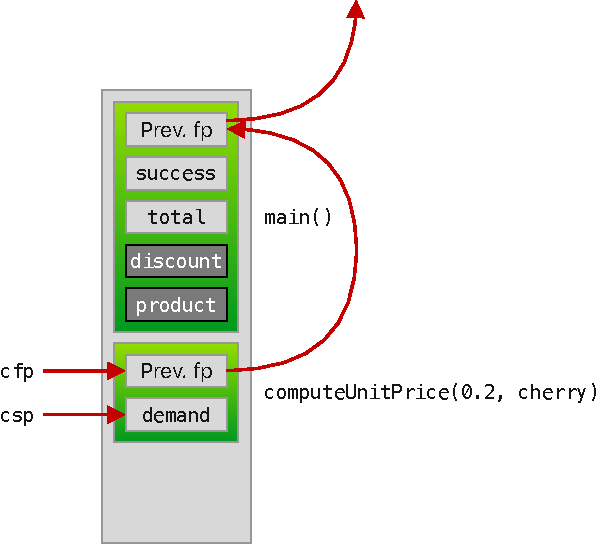
\includegraphics{Images/GCCC Stack.pdf}
	\caption{A call stack containing two call frames in a configuration of GCCC where no registers are available for storing parameters and local variables. The first call frame belongs to the initial procedure \texttt{main} which is called by the runtime, a dynamic linker, or the operating system and takes no parameters. Its call frame contains a \emph{previous frame pointer} capability that points to an unspecified location (possibly \texttt{null}) as well as two local variables \texttt{discount} and \texttt{price}. \texttt{main} invokes the 2-parameter \texttt{computeUnitPrice} procedure, binding the value \texttt{0.2} to the \texttt{discount} parameter and \texttt{cherry} to the \texttt{product} parameter. The latter procedure's call frame contains a \emph{previous frame pointer} capability that points to the location of the \emph{previous frame pointer} capability in the previous call frame, as well as a local variable \texttt{demand}. This call frame is at the top of the stack and so the \texttt{cfp} register's capability points to the \emph{previous frame pointer} capability in \texttt{computeUnitPrice}'s call frame. The \texttt{csp} register's capability always points to the last datum pushed on the stack, which is \texttt{demand} in this example. Note that the stack grows downward.}
	\label{fig:gcccstack}
\end{figure}

\paragraph{From CC to SV} CC introduces procedures with parameters and results. It is \lowered{} to its \g{lowerlang} SV (Structured Values) by imposing the \g{cc} described above. We'll work through the CC to SV \g{nanopass} by applying it to the following CC program.
\ilfile{Programs/42.cc}

The main program begins by pushing a new scope, which is essentially the same as pushing a new call frame to the call stack.\footnote{The term \emph{(location) scope} abstracts from the call frame. \Gs{il} above AL do not support accessing the call frame directly but do provide a way of creating and restoring sets of abstract locations, hence the term.}
\ilfile[lastline=3]{Programs/42.sv}

The program receives a \g{retcap} in \texttt{cra}, which it can use to return to the \g{rt} (or operating system). To free up this register for other uses, it binds its value to an abstract location.\footnote{\texttt{call} effects redefine the register. The register allocator will notice a conflict and thus assign the saved \g{retcap} to a location on the call frame. For leaf procedures, no such conflict occurs and the register allocator optimises away the binding to \texttt{cc.retcap}.}
\ilfile[firstline=4, lastline=4]{Programs/42.sv}

The \texttt{call} effect is \lowered{} by copying the arguments to the appropriate registers (or onto a newly stack-allocated arguments record for arguments that don't fit in registers), passing control to the callee, and finally (after control is returned) copying the result from \texttt{a0} to the result location. The register allocator (discussed in \cref{sct:id}) needs to know what registers are used for passing arguments and are thus live across the call; the \texttt{call} effect is therefore annotated with a list of used arguments registers.
\ilfile[firstline=5, lastline=8]{Programs/42.sv}

The program finishes by restoring the \g{retcap} (which it can only do while the current scope is valid), popping the current scope, then returning to the program's caller.
\ilfile[firstline=9, lastline=13]{Programs/42.sv}

The procedure begins analogously to the program by pushing a new scope and binding the caller's \g{retcap} to an abstract location. It does the same for all \gs{ceesaved}, since their contents must be preserved by a procedure before it can use them. The register allocator in a later \g{nanopass} cleans up (some) redundant moves.
\ilfile[firstline=14, lastline=21]{Programs/42.sv}

It then binds each received argument to a location with its corresponding parameter's name, making those arguments available to the rest of the procedure which expects arguments in those locations. This operation also frees the argument registers for other uses, such as for calls within the procedure.
\ilfile[firstline=22, lastline=23]{Programs/42.sv}

The rest of the procedure is left as-is.
\ilfile[firstline=24, lastline=24]{Programs/42.sv}

The \texttt{return} effect is \lowered{} by copying the result to the result register \texttt{a0}, restoring the contents of \gs{ceesaved} and the \g{retcap}, popping the current scope, and returning control back to the caller.
\ilfile[firstline=25]{Programs/42.sv}

\Cref{lst:42s} shows this program after a \g{lowering} to CHERI-RISC-V assembly (S), although the association between SV and S code may be unclear as there are many \gs{nanopass} between these \gs{il}.

\begin{listing}[ht]
	\asmfile[firstline=107, lastline=136]{Programs/42.s}
	\caption{An assembly excerpt of the 42 program, with the \texttt{sum} procedure starting from line 118. The current version of Glyco is unable to delete some redundant moves such as the ones in lines 121–126.}
	\label{lst:42s}
\end{listing}

\newpage

\section{Structured Values} \label{sct:sv}
\plfig[4]{v0.1 SV}

This section introduces vectors and records (collectively called \emph{structured values}) and the SV language.

\textbf{SV} (Structured Values) provides a structured abstraction over unstructured buffers in the form of vectors and records. A \textbf{vector} in SV is a homogeneous\footnote{All elements are of the same data type.} fixed-size\footnote{The number of elements is determined at creation and can only be changed by creating a new vector of the desired size and moving all elements to it.} array and is represented with a capability that points to the vector's first element, similarly to an array in the C programming language. A \textbf{record} is a heterogeneous\footnote{Values are not necessarily of the same data type.} key-value map with fixed keys and is similar to a C \texttt{struct}. However, unlike C \texttt{struct}s and like SV vectors, a record is represented by a capability that points to the record's first value. Vectors and records in SV are always passed by reference and never implicitly copied. Vector and record capabilities are automatically bounded to the region of memory they occupy; indexing a vector with an index that exceeds the vector's length causes a machine trap.\footnote{Due to CHERI-RISC-V bounds compression, a buffer capability may grant a larger region of memory than requested during allocation, meaning that some \enquote{out of bounds} indices near the end index may actually be valid and not cause a trap. Glyco compensates for this by allocating the extra memory granted by the buffer capability, thereby ensuring that no other buffer can occupy this extra space accessible by the first capability.}

\paragraph{From SV to ID} Structured values are implemented in the \g{lowerlang} ID (Inferred Declarations) by translating effects dealing with them into effects dealing with unstructured data buffers. For example, the SV program (with alternating effects highlighted)
\ilfile[highlightlines={4-10, 12, 14, 16, 18, 20}]{Programs/sequences.sv}
is \lowered{} to the following ID program (with the above highlighted effects' \gs{lowering} highlighted):
\ilfile[highlightlines={4, 6, 8, 11-12, 15-16, 19-20}]{Programs/sequences.id}

\section{Abstract Locations} \label{sct:id}
\plfig[9]{v0.1 ID}

This section sets out the difference between abstract and physical locations, register allocation, and the ID, AL, and ALA languages.

All programs until now have been able to bind values to names in one form or another, be it by using new named locations in effects or binding values to names with \texttt{let}. These names refer to physical locations where data can be stored, but without the programmer explicitly specifying the physical location itself, and are therefore referred to as \textbf{abstract locations}. The compiler is responsible for assigning each abstract location a \textbf{physical location} like a register or location in the call frame.

Since registers are orders of magnitude faster to access than locations in RAM, the compiler attempts to assign as many abstract locations as it can to registers in a process called \textbf{register allocation}. Since the number of registers is limited, the compiler may need to \textbf{spill} abstract locations to locations on the call frame. Glyco employs several heuristics to minimise the runtime cost by spilling abstract locations that it thinks will be accessed the least.

Glyco's register allocator is spread over three \gs{nanopass} which perform the following steps, for the main program and each procedure separately:
\begin{enumerate}
	\item Discover the abstract locations that are used and the data types that they take.
	\item For each abstract location, determine where in the program or procedure it is defined or redefined with a value and where that value is used. The execution path between a definition and that definition's last use is a \textbf{liveness interval}, a period of time where the definition's value is considered \emph{live}.
	\item Find out which liveness intervals overlap with other liveness intervals. The locations involved in such overlapping intervals are considered to be \textbf{in conflict} with each other.
	\item Assign registers to abstract locations so that no two abstract locations are assigned the same register if they are in conflict with each other. If no register is available for an abstract location, allocate space on the call frame and assign it that location.
	
	Prioritise abstract locations with few conflicts when assigning registers as they're likely to maximise the number of abstract locations that can be assigned to a register.
\end{enumerate}

A liveness example is shown in \cref{fig:liveness}.

\begin{SCfigure}
	\centering
	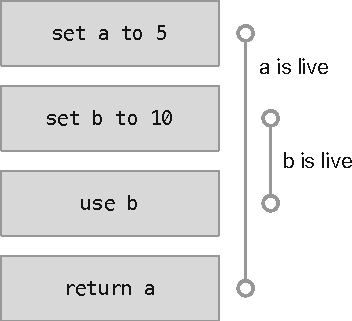
\includegraphics{Images/Liveness.pdf}
	\caption{A liveness example where $a$ and $b$ have overlapping liveness intervals and thus cannot be assigned to the same register. The conflict graph contains an edge between $a$ and $b$.}
	\label{fig:liveness}
\end{SCfigure}

\paragraph{From ID to AL} An ID program is \lowered{} to an AL (Abstract Locations) program by inferring a declaration for each abstract location used in the program and each of the program's procedures. Each declaration associates an abstract location with a data type. For example, the ID program
\ilfile{Programs/buffer.id}
is \lowered{} to the following AL program (declarations highlighted):
\ilfile[highlightlines={2}]{Programs/buffer.al}

\paragraph{From AL to ALA} Similar to how the previous \g{nanopass} infers local declarations, the AL to ALA (Abstract Locations, Annotated) \g{lowering} infers static\footnote{As observed from the code itself, without running or simulating the program.} liveness and conflict information about the program, and associates it with every effect and predicate in an ALA program. It consists of two data structures: a liveness set and a conflict graph.

An effect's \textbf{liveness set at entry} is a set of locations that are \textbf{possibly live} right before the effect is executed. Every location that is not in the set is considered \textbf{definitely dead}.\footnote{We choose to explicitly qualify liveness with \enquote{possibly} or \enquote{definitely} because by Rice's theorem it is impossible to ascertain whether a value is actually live in all execution paths. Liveness is a property of a program: a definition's value may not ever be live if the effects using the value are never executed. Compilers (including Glyco) take a conservative approach and \emph{assume} that a value is live if they cannot rule out that it is dead. This heuristic may cause suboptimal register allocation due to excessive liveness intervals, but guarantees correctness by not accidentally assigning two live values to the same register. In contrast, when an effect overwrites a location's value (without using the previous value), we can be certain about the previous value being dead at the point of entering the effect.} An effect's \textbf{conflict graph at entry} is a undirected graph of locations with an edge connecting every pair of locations that are in conflict right before the effect is executed. An effect's \textbf{liveness set at exit} resp. \textbf{conflict graph at exit} is the next effect's liveness set at entry resp. conflict graph at entry.

The analysis algorithm derives an effect's liveness set and conflict graph \emph{at entry} from the effect's liveness set and conflict graph \emph{at exit} using the following 2 rules.

\begin{itemize}
	
	\item If an effect \textbf{defines} a location's value, the location is marked as (definitely) dead at entry and thus removed from the liveness set at entry. We know for certain that the location is not live right before the effect executes since its value is overwritten.
	
	Additionally, the newly defined location is in conflict with all locations that are in the liveness set at exit. The effect (possibly) starts a liveness interval for the newly defined location in the middle of liveness intervals of each location in the liveness set. These liveness intervals overlap; the conflict graph at entry is therefore updated with edges between the newly defined location and every location in the liveness set at exit.
	
	\item If an effect \textbf{uses} a location's value, the location is marked as (possibly) live at entry and is thus added to the liveness set at entry. An effect that defines and uses the same location's value, i.e., an assignment to itself, is considered to keep the location (possibly) live.
	
\end{itemize}

Since the liveness set and conflict graph at entry depend on the liveness set and conflict graph at exit, the algorithm traverses the program backwards, i.e., against the direction of execution and towards the beginning of the program or procedure. The algorithm starts with an empty initial liveness set and conflict graph, i.e., a \texttt{return} effect's liveness set and conflict graph at exit are empty.

\paragraph{Location coalescing} The number of locations in a program can often be reduced by merging locations that are assigned the same value and are not in conflict with each other. For example, \iil/three/ and \iil/number/ in
\ilfile[highlightlines={6}]{Programs/coalescable.al}
can be coalesced to get
\ilfile{Programs/coalesced.al}
thereby saving one \texttt{set} effect (highlighted in the pre-coalescing example) and making the liveness set and conflict graph smaller.

The location coalescing optimisation algorithm works as follows:
\begin{enumerate}
	\item Select a candidate pair that is involved in a \texttt{set} effect. The algorithm is done if there are no (non-rejected) candidate pairs.
	\item If the candidate locations are in conflict with each other, reject the pair and try another.
	\item Tentatively form the union of the location vertices in the conflict graph. If the degree of the merged vertex is equal to or larger than the number of available registers, reject the pair and try another. This conservative heuristic by \citet{briggs} ensures that the merged location will not require spilling (to the call frame) after merging if the individual locations themselves do not require spilling.
	\item Commit the union of the location vertices in the conflict graph, arbitrarily choose which location to retain, and remove the other location from the program by substituting it everywhere with the retained location. If the pair consists of a physical and an abstract location,\footnote{Usually a result of the CC to SV \g{nanopass} which puts arguments and results in dedicated registers.} retain the physical location.
	\item Repeat from Step 1.
\end{enumerate}

\paragraph{From ALA to CD} The \g{nanopass} from ALA to CD (Conditionals) uses the conflict graph at entry of the program and of each procedure to determine an assignment of abstract locations to physical locations, and substitutes each abstract locations with its assigned physical location.

Register assignment is a graph colouring problem on the conflict graph where the colours are the available registers. No two connected locations in the conflict graph can be coloured with the same colour, i.e., no two locations that are in conflict can be assigned to the same register. The register assignment algorithm works as follows:
\begin{enumerate}
	\item Select an abstract location $L$ with the lowest degree and without an assigned physical location. The algorithm is done if there is no such location.
	\item Select an available register. If any abstract location already assigned to this register is in conflict with $L$, reject the register and try another. If no (non-rejected) register is available, spill the abstract location by assigning it a free location on the call frame.
	\item Repeat from Step 1.
\end{enumerate}

Unlike most algorithms in the compiler's \gs{nanopass}, this algorithm runs in $O(nm)$ time for $n$ locations and $m$ assignable registers,\footnote{Assuming that conflict graph queries are done in amortised constant time, as in Glyco.} which underlines the importance of minimising the number of abstract locations via optimisations such as location coalescing.

\section{Structured Jumps \& Branches} \label{sct:cd}
This section deals with the final major abstractions over straight-line programs: conditionals (\texttt{if}-\texttt{then}-\texttt{else} effects), sequences (\texttt{do} effects), and procedures. The \gs{nanopass} from the CD to BB languages linearise programs.

\plfig[8]{v0.1 CD}

In CD, a \textbf{conditional} consists of a predicate, an affirmative branch, and a negative branch. Whenever the predicate evaluates to true, the affirmative branch is executed, otherwise the negative branch is executed. A \textbf{sequence} sequentially executes its contained effects. A \textbf{procedure} can be invoked with a \texttt{call} effect which updates the \texttt{cra} register with the address of the next effect, then jumps to the procedure's code. These three features make CD a block-structured programming language. The upcoming \gs{nanopass} get programs to a form that can be readily translated into assembly.

\paragraph{From CD to PR} The CD to PR (Predicates) \g{nanopass} flattens conditionals, sequences, and procedures into \gs{bblock}. A \textbf{\g{bblock}} is a labelled sequence of effects that is executed from beginning to end, before jumping or branching to itself or to other blocks. No effect in the block but the first is labelled. A \g{bblock}'s effects are followed by a \textbf{continuation}, which is a jump, branch, or call. No effect except the continuation is a jump, call, or branch. For example, the CD program (code belonging to every even \g{bblock} highlighted)
\ilfile[highlightlines={3-5, 9-10, 12-15}]{Programs/ifproc.cd}
is \lowered{} to the PR program (every even \gs{bblock} highlighted)
\ilfile[highlightlines={2-6, 8-12, 14-18}, tabsize=1]{Programs/ifproc.pr}

This program can be presented as a control-flow graph like in \cref{fig:cfg} where the edges are transitions specified by continuations and vertices are either basic blocks or (implied) callers. The graph contains one connected subgraph for the main program and for each procedure. Control jumps from one subgraph to another via \texttt{call} and \texttt{return} continuations. Each \texttt{branch} continuation specifies two outgoing edges.
\begin{SCfigure}[][ht]
	\centering
	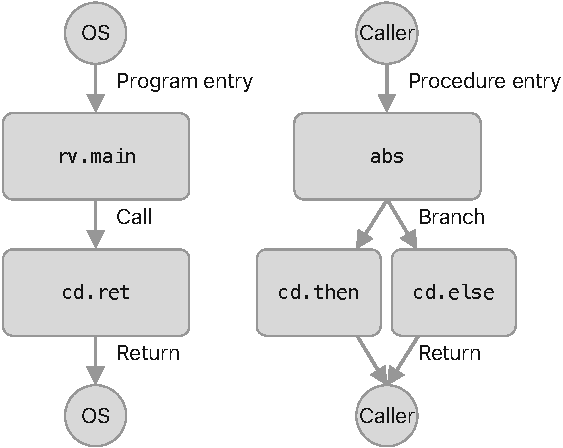
\includegraphics{Images/Basic Blocks.pdf}
	\caption{A control-flow graph of the PR program. The connected graph on the left represents the main program whereas the one on the right represents the \texttt{abs} procedure.}
	\label{fig:cfg}
\end{SCfigure}

\paragraph{From PR to BB} The next \g{il}, BB (Basic Blocks), does not support predicates so the PR to BB \g{nanopass} maps predicates to appropriate continuations. For example, the above program is \lowered{} to the BB program
\ilfile{Programs/ifproc.bb}

\paragraph{From BB to FO} The final structural transformation linearises \gs{bblock} in BB programs to get an FO (Flexible Operands) program with a single list of unlabelled and labelled effects.

The \g{nanopass} attempts to get an optimal placement of \gs{bblock}, i.e., an optimal trace, by juxtaposing successive blocks where possible. Unconditional jumps between juxtaposed blocks can be elided thereby avoiding the cost associated with jumps such as redundant instructions and pipeline stalls.

The above BB program becomes the FO program in \cref{lst:ifproc-fo}.
\begin{listing}[ht]
	\ilfile{Programs/ifproc.fo}
	\caption{An FO program.}
	\label{lst:ifproc-fo}
\end{listing}

\section{Basic Abstractions over Assembly} \label{sct:fo}
\plfig[14]{v0.1 FO}

This section briefly discusses the last \gs{il}, which provide some useful basic abstractions over the CHERI-RISC-V instruction set.

\paragraph{From FO to MM} FO effects accept input from several kinds of sources such as constants, registers, and (call) frame locations; and can produce results in registers or frame locations. Some source–destination combinations are not available as CHERI-RISC-V instructions. There is for instance no addition instruction that can load operands from memory or store a result in memory. There's also no subtraction instruction that takes an immediate minuend (first term).

To abstract this complexity away in FO and higher \gs{il}, the FO to MM (Managed Memory) \g{nanopass} inserts the necessary loads and stores and reorders operands to realise an effect using CHERI-RISC-V instructions in a lower \g{nanopass}.

\paragraph{From MM to RV} MM introduces the call stack, the heap, and operations on them.

The MM to RV (CHERI-RISC-V) \g{nanopass} translates call frame operations such as \texttt{pushFrame}, \texttt{popFrame}, \texttt{load}, and \texttt{store} into manipulations of the stack capability register \texttt{csp} and frame capability register \texttt{cfp}.

Buffer allocation is implemented using a dedicated heap capability register \texttt{ctp}. The heap capability points to the next free location on the heap and allocation increases the heap capability address — deallocation is not supported.

\paragraph{From RV to S} An RV program consists of CHERI-RISC-V instructions. The RV to S (CHERI-RISC-V Assembly) \g{nanopass} serialises these instructions. For example, the \iil/copyWord(destination: a0, source: a1)/ instruction is serialised as \iasm/mv a0, a1/.

\Cref{lst:ifproc-s} shows an S program derived from the FO program in \cref{lst:ifproc-fo}.

\begin{listing}[ht]
	\asmfile[firstline=107, lastline=119]{Programs/ifproc.s}
	\caption{The S program from the FO program in \cref{lst:ifproc-fo}, excluding runtime code.}
	\label{lst:ifproc-s}
\end{listing}

\paragraph{From S to ELF} The final step of the compiler pipeline is assembling and linking. These two steps are delegated to the assembler from the CHERI LLVM compiler toolchain.\footnote{This last step is unrelated to the research problem, hence this dependency on LLVM.} The result is an ELF file that, depending on the compilation target, can be executed in either the Sail-based CHERI-RISC-V emulator or in CheriBSD.

\biblio{}
\onlyinsubfile{\glsaddall\printglossaries}
\end{document}
